\documentclass[conference]{IEEEtran}
\usepackage{cite}
\usepackage{amsmath,amssymb}
\usepackage{graphicx}
\usepackage{booktabs}
\usepackage{url}
\usepackage{tikz}
\usetikzlibrary{arrows.meta}

\begin{document}

\title{Systolic Array Matrix Multiplication Accelerator:\\A Parameterised Verilog Implementation}

\author{
\IEEEauthorblockN{Anurag Kumar\IEEEauthorrefmark{1},
Augustya Purohit\IEEEauthorrefmark{2},
Harsh Raj\IEEEauthorrefmark{3},
Sumit Yadav\IEEEauthorrefmark{4} and
Adil Mirza\IEEEauthorrefmark{5}}
\IEEEauthorblockA{Newton School of Technology, Rishihood University, Sonipat, India\\
Modern Computer Architecture --- Team MCA\_Project\_2024\_C\_Team1 (Section C)\\
Enrolment Nos.: \IEEEauthorrefmark{1}2401010088,
\IEEEauthorrefmark{2}2401010114,
\IEEEauthorrefmark{3}2401010180,
\IEEEauthorrefmark{4}2401010464,
\IEEEauthorrefmark{5}2401020005\\
\{anurag.kumar2024, augustya.purohit2024, harsh.raj2024, sumit.yadav2024, adil.mirza2024\}@nst.rishihood.edu.in}
}

\maketitle

\begin{abstract}
Matrix multiplication dominates the run time of machine-learning inference,
signal processing and scientific workloads, yet a general-purpose processor
executes its $N^3$ multiply-accumulate operations essentially one after another.
This report presents the Phase~I prototype of a systolic array accelerator that
computes $C = A \times B$ for $N \times N$ signed integer matrices. The design
is a two-dimensional mesh of $N^2$ identical processing elements, each
containing one multiplier, one adder and three registers, connected only to
their nearest neighbours. Operands are injected along the left and top edges
with a diagonal skew so that matching elements meet in the correct cell at the
correct cycle. The accelerator is written in synthesisable, fully parameterised
Verilog-2005 and verified with a self-checking testbench against a behavioural
reference model. For array sizes $N = 2$ to $16$ every directed and random test
passes, and the measured latency is exactly $3N-1$ clock cycles, compared with
$N^3$ cycles for a single multiply-accumulate datapath.
\end{abstract}

\begin{IEEEkeywords}
systolic array, matrix multiplication, hardware accelerator, Verilog, RTL,
processing element, AI hardware
\end{IEEEkeywords}

\section{Introduction}
The end of Dennard scaling has moved computer architecture towards
domain-specific accelerators, which gain efficiency by matching the hardware
structure to the structure of one important computation \cite{hennessy}. Dense
matrix multiplication is the most valuable such computation: fully connected
and convolutional neural-network layers, digital filters and linear solvers all
reduce to it \cite{sze}.

For two $N \times N$ matrices the product is
\begin{equation}
C_{ij} = \sum_{k=0}^{N-1} A_{ik} B_{kj}, \qquad 0 \le i,j < N,
\label{eq:matmul}
\end{equation}
which needs $N^3$ multiply-accumulate (MAC) operations. On a scalar processor
these are serialised through one arithmetic unit and every operand is fetched
from memory, so performance is limited by both computation and memory traffic.

A systolic array removes both limits. It is a regular grid of simple cells that
compute in parallel and pass data only to adjacent cells on every clock tick,
much as the heart pumps blood in rhythmic pulses \cite{kung1982}. Each operand
is read from memory once and then reused by a whole row or column of cells as it
travels through the grid.

The objective of this project is to design, implement and verify such an
accelerator at the register-transfer level. Phase~I, reported here, delivers a
working and verified RTL prototype together with its verification environment.

\section{Literature Review}
Kung and Leiserson introduced systolic arrays as an architecture suited to
VLSI, in which a few types of simple cells are replicated and connected by
short, local wires \cite{kungleiserson}. Kung later argued that this style
gives simple and regular designs, high concurrency and a balance between
computation and input/output, which makes it attractive for compute-bound
algorithms such as matrix arithmetic \cite{kung1982}. S.~Y.~Kung formalised the
design procedure: an algorithm is written as a dependence graph and then mapped
to an array by choosing a projection direction and a linear schedule
\cite{sykung}. The architecture used in this work corresponds to mapping the
three-dimensional dependence graph of \eqref{eq:matmul} along the $k$ axis, so
that each cell owns one output element.

Interest in systolic arrays returned with deep learning. Google's Tensor
Processing Unit is built around a matrix multiply unit of $256 \times 256$
8-bit MAC cells and reports large gains in performance per watt over
contemporary CPUs and GPUs for inference \cite{tpu}. Gemmini provides an
open-source generator of systolic-array accelerators integrated with RISC-V
processors, allowing the full hardware--software stack to be evaluated
\cite{gemmini}. Wei \emph{et al.} generate systolic arrays for convolutional
networks on FPGAs automatically from a high-level description \cite{wei}.
Eyeriss shows a related spatial architecture in which a grid of processing
elements with local data reuse reduces memory accesses, the dominant energy
cost \cite{eyeriss}. Sze \emph{et al.} survey these approaches and identify
operand reuse and local communication as the common source of efficiency
\cite{sze}.

The surveyed systems are large and target full neural networks. This project
isolates the core idea in a compact, parameterised and openly verifiable RTL
design, suitable for studying the latency, area and scheduling trade-offs
covered in a computer architecture course.

\section{Proposed Solution}
\subsection{Architecture Overview}
The accelerator (Fig.~\ref{fig:array}) consists of three Verilog modules:
\texttt{pe}, the processing element; \texttt{systolic\_array}, an $N \times N$
mesh of processing elements built with \texttt{generate} loops; and
\texttt{matmul\_accel}, the top level containing the controller and the skewed
input feeders. The matrix size $N$, operand width \texttt{DATA\_W} and
accumulator width \texttt{ACC\_W} are parameters.

\begin{figure}[t]
\centering
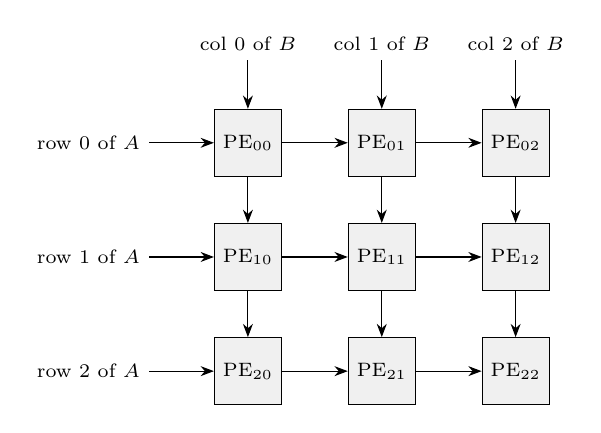
\begin{tikzpicture}[>=Stealth, font=\scriptsize,
  pe/.style={draw, fill=gray!12, minimum size=8.5mm, inner sep=0pt}]
\foreach \i in {0,1,2} {
  \foreach \j in {0,1,2} {
    \node[pe] (pe\i\j) at (\j*1.7, -\i*1.45) {PE$_{\i\j}$};
  }
}
\foreach \i in {0,1,2} {
  \draw[->] (-1.25, -\i*1.45) node[left] {row \i{} of $A$} -- (pe\i0);
  \draw[->] (pe\i0) -- (pe\i1);
  \draw[->] (pe\i1) -- (pe\i2);
}
\foreach \j in {0,1,2} {
  \draw[->] (\j*1.7, 1.05) node[above] {col \j{} of $B$} -- (pe0\j);
  \draw[->] (pe0\j) -- (pe1\j);
  \draw[->] (pe1\j) -- (pe2\j);
}
\end{tikzpicture}
\caption{Systolic mesh for $N=3$. Operands of $A$ travel left to right and
operands of $B$ travel top to bottom; PE$_{ij}$ accumulates $C_{ij}$.}
\label{fig:array}
\end{figure}

\subsection{Processing Element}
Each processing element has two operand inputs, $a_{in}$ from the left and
$b_{in}$ from the top, and holds three registers. On every enabled clock edge
it performs
\begin{align}
acc &\leftarrow acc + a_{in} \cdot b_{in}, \nonumber\\
a_{out} &\leftarrow a_{in}, \qquad b_{out} \leftarrow b_{in}.
\end{align}
The cell therefore computes one MAC per cycle and forwards both operands
unchanged to its right and bottom neighbours. Because all wires are
nearest-neighbour, the critical path is one multiplier followed by one adder
and does not grow with $N$.

\subsection{Input Skewing and Scheduling}
For PE$_{ij}$ to compute \eqref{eq:matmul}, $A_{ik}$ and $B_{kj}$ must arrive
together. An operand entering row $i$ needs $j$ cycles to reach column $j$, and
an operand entering column $j$ needs $i$ cycles to reach row $i$. The feeders
therefore delay row $i$ of $A$ by $i$ cycles and column $j$ of $B$ by $j$
cycles: at cycle $t$ the left edge of row $i$ receives $A_{i,\,t-i}$ and the top
edge of column $j$ receives $B_{t-j,\,j}$, with zeros outside the valid range.
Both operands with index $k$ then meet in PE$_{ij}$ at cycle
\begin{equation}
t = i + j + k .
\end{equation}
The last product is formed in PE$_{N-1,N-1}$ at $t = 3N-3$, so the computation
needs $3N-2$ cycles, plus one cycle to latch the operands.

\subsection{Controller}
A two-state controller sequences the operation. On \texttt{start} it latches
both matrices, clears all accumulators and enters the run state, where a cycle
counter drives the feeders. When the counter reaches $3N-3$ it raises
\texttt{done}, which stays high until the next \texttt{start}; the results
remain stable in the accumulators.

\subsection{Bit-Width Selection}
With $W$-bit signed operands the largest product magnitude is $2^{2W-2}$ and
each accumulator sums $N$ products, so overflow is impossible when
\begin{equation}
\texttt{ACC\_W} \ge 2W + \lceil \log_2 N \rceil .
\end{equation}
The default configuration ($W = 8$, \texttt{ACC\_W} $= 24$) is therefore safe
for arrays up to $N = 256$.

\section{Prototype and Results}
The prototype is simulated with Icarus Verilog \cite{iverilog}. The
self-checking testbench loads matrices, pulses \texttt{start}, waits for
\texttt{done} and compares all $N^2$ outputs with a behavioural triple-loop
model of \eqref{eq:matmul}. Each run applies four directed tests (identity,
counting pattern, all operands at the most negative value, and mixed-sign
extremes) followed by 100 back-to-back random multiplications, which also
checks that the array is cleared correctly between operations.

All 104 tests pass for $N = 2, 3, 4, 5, 8$ and $16$ with 8-bit operands, and
for $N = 4$ with 16-bit operands. Table~\ref{tab:results} lists the latency
measured in simulation. The last two columns compare cycle counts with an
idealised datapath that has a single MAC unit and needs $N^3$ cycles; this is an
analytical comparison, not a measurement of a real processor.

\begin{table}[t]
\caption{Measured Latency of the Prototype (8-bit Operands)}
\label{tab:results}
\centering
\begin{tabular}{ccccc}
\toprule
$N$ & PEs & Latency & Single-MAC & Cycle-count \\
    & ($N^2$) & (cycles) & ($N^3$ cycles) & ratio \\
\midrule
2  & 4   & 5  & 8    & 1.6$\times$ \\
4  & 16  & 11 & 64   & 5.8$\times$ \\
8  & 64  & 23 & 512  & 22.3$\times$ \\
16 & 256 & 47 & 4096 & 87.1$\times$ \\
\bottomrule
\end{tabular}
\end{table}

The measured latency equals $3N-1$ in every case, matching the schedule
derived in Section~III. The cost of this speed is area: the design uses $N^2$
multipliers. Synthesis results (area, maximum frequency and power) have not yet
been obtained and are planned for Phase~II.

\section{Individual Contributions}
Table~\ref{tab:contrib} lists the responsibility of each team member in
Phase~I.

\begin{table}[t]
\caption{Individual Contributions}
\label{tab:contrib}
\centering
\begin{tabular}{p{2.7cm}p{5.1cm}}
\toprule
Member & Contribution \\
\midrule
Anurag Kumar (Team Lead) & Overall architecture; top-level controller and
input skew scheduling (\texttt{matmul\_accel}); repository and integration. \\
Augustya Purohit & Processing element design (\texttt{pe}); signed arithmetic
and bit-width analysis. \\
Harsh Raj & Parameterised $N \times N$ mesh (\texttt{systolic\_array}) and
interconnect structure. \\
Sumit Yadav & Verification: self-checking testbench, reference model, test
plan and waveform analysis. \\
Adil Mirza & Literature review, block diagrams, project report and prototype
demonstration video. \\
\bottomrule
\end{tabular}
\end{table}

\section{Conclusion and Future Work}
Phase~I delivers a parameterised systolic array matrix multiplier in Verilog
that is verified bit-exactly against a reference model for six array sizes and
two operand widths, with a latency of $3N-1$ cycles. In Phase~II we plan to
synthesise the design for an FPGA to obtain area, timing and power figures; add
a streaming memory-mapped interface so that operands need not be presented in
parallel; support rectangular matrices; pipeline the multiplier to raise the
clock frequency; and compare the accelerator against a sequential single-MAC
baseline implemented in the same flow.

\begin{thebibliography}{00}
\bibitem{kungleiserson} H.~T.~Kung and C.~E.~Leiserson, ``Systolic arrays (for
VLSI),'' in \emph{Sparse Matrix Proceedings 1978}. Philadelphia, PA, USA: SIAM,
1979, pp.~256--282.
\bibitem{kung1982} H.~T.~Kung, ``Why systolic architectures?,''
\emph{Computer}, vol.~15, no.~1, pp.~37--46, Jan.~1982.
\bibitem{sykung} S.~Y.~Kung, \emph{VLSI Array Processors}. Englewood Cliffs,
NJ, USA: Prentice-Hall, 1988.
\bibitem{tpu} N.~P.~Jouppi \emph{et al.}, ``In-datacenter performance analysis
of a tensor processing unit,'' in \emph{Proc. 44th Annu. Int. Symp. Comput.
Archit. (ISCA)}, 2017, pp.~1--12.
\bibitem{gemmini} H.~Genc \emph{et al.}, ``Gemmini: Enabling systematic
deep-learning architecture evaluation via full-stack integration,'' in
\emph{Proc. 58th ACM/IEEE Design Autom. Conf. (DAC)}, 2021, pp.~769--774.
\bibitem{wei} X.~Wei \emph{et al.}, ``Automated systolic array architecture
synthesis for high throughput CNN inference on FPGAs,'' in \emph{Proc. 54th
ACM/EDAC/IEEE Design Autom. Conf. (DAC)}, 2017, pp.~1--6.
\bibitem{eyeriss} Y.-H.~Chen, T.~Krishna, J.~S.~Emer, and V.~Sze, ``Eyeriss: An
energy-efficient reconfigurable accelerator for deep convolutional neural
networks,'' \emph{IEEE J. Solid-State Circuits}, vol.~52, no.~1, pp.~127--138,
Jan.~2017.
\bibitem{sze} V.~Sze, Y.-H.~Chen, T.-J.~Yang, and J.~S.~Emer, ``Efficient
processing of deep neural networks: A tutorial and survey,'' \emph{Proc. IEEE},
vol.~105, no.~12, pp.~2295--2329, Dec.~2017.
\bibitem{hennessy} J.~L.~Hennessy and D.~A.~Patterson, \emph{Computer
Architecture: A Quantitative Approach}, 6th~ed. Cambridge, MA, USA: Morgan
Kaufmann, 2017.
\bibitem{iverilog} S.~Williams, ``Icarus Verilog.'' [Online]. Available:
\url{https://steveicarus.github.io/iverilog/}
\end{thebibliography}

\end{document}
